\documentclass{beamer}


\usepackage[utf8]{inputenc}
\usepackage{amsmath}
\usepackage{amsfonts}
\usepackage{amssymb}
\usepackage{subcaption}
\usepackage{graphicx}
\usepackage{ragged2e}  % `\justifying` text
\usepackage{booktabs}  % Tables
\usepackage{tabularx}
\usepackage{tikz}      % Diagrams
\usetikzlibrary{calc, shapes, backgrounds}
\usepackage{amsmath}
\usepackage{amssymb}
\usepackage{listings}  % Code listings
\usepackage[T1]{fontenc}
\usepackage{url}       % `\url
\usepackage{dsfont}
\usepackage{hyperref}
\usepackage{multicol}
\usepackage{hyperref}
\usepackage{listings}
\usepackage{booktabs} % Required for better horizontal rules in tables
\usepackage{multirow}

\usepackage{xcolor} %https://en.wikibooks.org/wiki/LaTeX/Colors

\usepackage{theme/beamerthemehbrs}

\author[Enriquez, Kramer, Massey]{Angela Enriquez, Erick Kramer, Ethan Massey}
\title{MAAS Project}
\subtitle{Flying Saucers Bakery}
\institute[HBRS]{Hochschule Bonn-Rhein-Sieg}
\date{23.01.2019}
%\subject{Pitch}

% \thirdpartylogo{path/to/your/image}


\begin{document}
	
		\begin{frame}
			\titlepage
		\end{frame}
		
		\begin{frame}
			\frametitle{System architecture}
			\begin{figure}
				\centering
				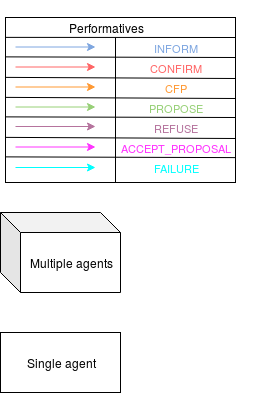
\includegraphics[scale=0.4]{images/conventions.png}
				\caption{Architecture of the Bakery JADE multi-agent system.}
				\label{fig:architecture}
			\end{figure}
		\end{frame}
		
		\begin{frame}
			\frametitle{System architecture}
			\begin{figure}\vspace{-1cm}
				\centering
				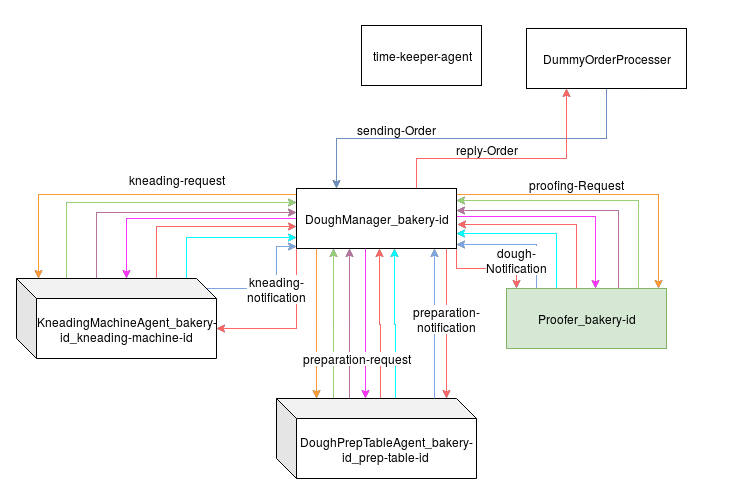
\includegraphics[scale=0.4]{images/doughStage.png}
				\caption{Architecture of the Bakery JADE multi-agent system.}
				\label{fig:architecture}
			\end{figure}
		\end{frame}
		
		\begin{frame}
			\frametitle{System architecture}
			\begin{figure} \vspace{-1cm}
				\centering
				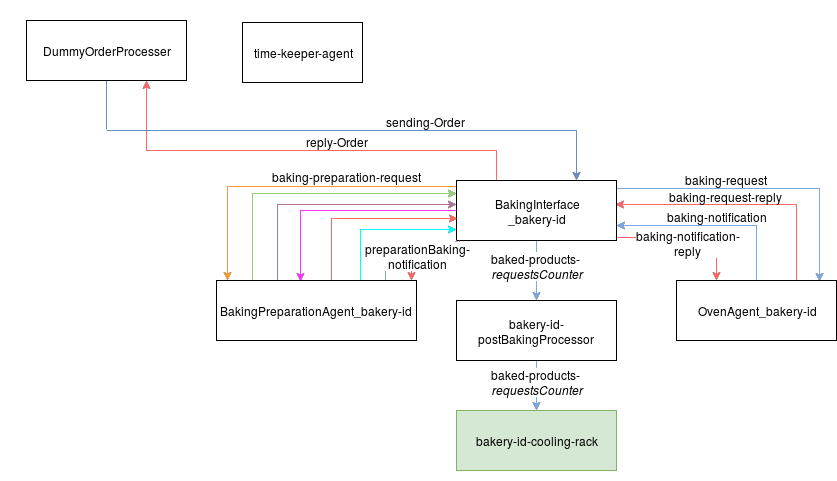
\includegraphics[scale=0.38]{images/bakingStage.png}
				\caption{Architecture of the Bakery JADE multi-agent system.}
				\label{fig:architecture}
			\end{figure}
		\end{frame}
		
		\begin{frame}
			\frametitle{Agents}
			\begin{table}[h!]	
				\centering
				\tiny
				
				\begin{tabular}{llll}
					\toprule   
					
					Production Stage & Agent  & Created by & Number of instances \\
					\midrule
					
					\multirow{1}{*} {Order Processing} &
					
					{DummyOrderProcesser} &
					
					DoughPrepStageInitializer & 1 \\
					
					
					\cmidrule(l){1-4}
					
					\multirow{7}{*} {Dough Preparation} &
					
					{DoughManager} &
					
					DoughPrepStageInitializer & 1 per bakery ID \\
					
					\cmidrule(l){2-4} 
					
					{} & KneadingMachineAgent & DoughManager & {\shortstack[l]{$n$ per bakery ID, where $n$ \\ is taken from bakeries.json}} \\
					
					\cmidrule(l){2-4} 
					
					{} & DoughPrepTableAgent & DoughManger & {\shortstack[l]{$n$ per bakery ID, where $n$ \\ is taken from bakeries.json}} \\
					
					\cmidrule(l){2-4} 
					
					{} & Proofer & DoughPrepStageInitializer &  1 per bakery ID \\
					
					\midrule
					
					\multirow{7}{*} {Baking} &
					
					{BakingInterface} &
					
					BakingMasMaasInitializer & 1 per bakery ID \\
					
					\cmidrule(l){2-4} 
					
					{} & OvenAgent & BakingInterface & 1 per bakery ID \\
					
					\cmidrule(l){2-4} 
					
					{} & BakingPreparationAgent & BakingInterface & 1 per bakery ID \\
					
					\cmidrule(l){2-4} 
					
					{} & PostBakingProcessor & BakingInterface &  1 per bakery ID \\
					
					\cmidrule(l){2-4} 
					
					{} & CoolingRackAgent & BakingStageInitializer &  1 per bakery ID \\
					
					\bottomrule
				\end{tabular}
				\caption{Agents in the Bakery JADE.} 
				\label{table-agents}
			\end{table}
			
		\end{frame}
		
		\begin{frame}
			\frametitle{Behaviours}
			\begin{table}[h!]	
				\centering
				\tiny				
				\begin{tabular}{llll}
					\toprule   
					
					Production Stage & Agent  & Behaviour Name & Behaviour Type \\
					\midrule
					
					\multirow{2}{*} {Order Processing} &
					
					\multirow{2}{*} {DummyOrderProcesser} &
					
					timeTracker & CyclicBehaviour \\
					
					\cmidrule(l){3-4}
					
					{} & {} & sendOrder & Behaviour \\
					
					\cmidrule(l){1-4}
					
					\multirow{15}{*} {Dough Preparation} &
					
					\multirow{15}{*} {Dough Manager} &
					
					timeTracker & CyclicBehaviour \\
					
					\cmidrule(l){3-4}
					
					{} & {} & ReceiveOrders & CyclicBehaviour \\
					
					\cmidrule(l){3-4}
					
					{} & {} & checkingKneadingWorkqueue & CyclicBehaviour \\
					
					\cmidrule(l){3-4}
					
					{} & {} & checkingPreparationWorkqueue & CyclicBehaviour \\
					
					\cmidrule(l){3-4}
					
					{} & {} & checkingProofingWorkqueue & CyclicBehaviour \\
					
					\cmidrule(l){3-4}
					
					{} & {} & RequestKneading & Behaviour \\
					
					\cmidrule(l){3-4}
					
					{} & {} & RequestPreparation & Behaviour \\
					
					\cmidrule(l){3-4}
					
					{} & {} & RequestProofing & Behaviour \\
					
					\cmidrule(l){3-4}
					
					{} & {} & ReceiveKneadingNotification & CyclicBehaviour \\
					
					\cmidrule(l){3-4}
					
					{} & {} & ReceivePreparationNotification & CyclicBehaviour \\
					
					
					\bottomrule
				\end{tabular}
				\caption{Behaviours in the Bakery JADE. Part 1.} 
				\label{table-behaviours1}
			\end{table}
		\end{frame}
		
		\begin{frame}
			\frametitle{Behaviours}
			\begin{table}[h!]	
				\centering
				\tiny				
				\begin{tabular}{llll}
					\toprule   

					Production Stage & Agent  & Behaviour Name & Behaviour Type \\
					\midrule
					
					\multirow{15}{*} {Dough Preparation} &
					
					 \multirow{7}{*} {KneadingMachineAgent} &
					
					timeTracker & CyclicBehaviour \\
					
					\cmidrule(l){3-4}
					
					{} & {} & ReceiveProposalRequests & CyclicBehaviour \\
					
					\cmidrule(l){3-4}
					
					{} & {} & ReceiveKneadingRequests & CyclicBehaviour \\
					
					\cmidrule(l){3-4}
					
					{} & {} & Kneading & OneShotBehaviour \\
					
					\cmidrule(l){3-4}
					
					{} & {} & SendKneadingNotification & Behaviour \\
					
					\cmidrule(l){2-4}
					
					{} & \multirow{7}{*} {DoughPrepTableAgent} &
					
					timeTracker & CyclicBehaviour \\
					
					\cmidrule(l){3-4}
					
					{} & {} & ReceiveProposalRequests & CyclicBehaviour \\
					
					\cmidrule(l){3-4}
					
					{} & {} & ReceivePreparationRequests & CyclicBehaviour \\
					
					\cmidrule(l){3-4}
					
					{} & {} & Preparation & OneShotBehaviour \\
					
					\cmidrule(l){3-4}
					
					{} & {} & SendPreparationNotification & Behaviour \\
					
					\cmidrule(l){2-4}
					
					{} & \multirow{7}{*} {Proofer} &
					
					timeTracker & CyclicBehaviour \\
					
					\cmidrule(l){3-4}
					
					{} & {} & ReceiveProposalRequests & CyclicBehaviour \\
					
					\cmidrule(l){3-4}
					
					{} & {} & ReceiveProofingRequests & CyclicBehaviour \\
					
					\cmidrule(l){3-4}
					
					{} & {} & Proofing & OneShotBehaviour \\
					\cmidrule(l){3-4}
					
					{} & {} & SendDoughNotification & Behaviour \\
					
					\bottomrule
				\end{tabular}
				\caption{Behaviours in the Bakery JADE. Part 2.} 
				\label{table-behaviours1}
			\end{table}
		\end{frame}
		
		\begin{frame}
			\frametitle{Behaviours}
			
			\begin{table}[h!]\vspace{-0.5cm}	
				\centering
				\tiny
				
				\begin{tabular}{llll}
					\toprule   
					
					Production Stage & Agent  & Behaviour Name & Behaviour Type \\
					\midrule
					
					\multirow{25}{*} {Baking} &
					
					\multirow{13}{*} {BakingInterface} &
					
					timeTracker & CyclicBehaviour \\
					
					\cmidrule(l){3-4}
					
					{} & {} & ReceiveOrders & CyclicBehaviour \\
					
					\cmidrule(l){3-4}
					
					{} & {} & ReceiveDoughNotification & CyclicBehaviour \\
					
					\cmidrule(l){3-4}
					
					{} & {} & checkingBakingWorkqueue & CyclicBehaviour \\
					
					\cmidrule(l){3-4}
					
					{} & {} & checkingPreparationWorkqueue & CyclicBehaviour \\
					
					\cmidrule(l){3-4}
					
					{} & {} & RequestBaking & Behaviour \\
					
					\cmidrule(l){3-4}
					
					{} & {} & RequestPreparation & Behaviour \\
					
					\cmidrule(l){3-4}
					
					{} & {} & RequestCooling & Behaviour \\
					
					\cmidrule(l){3-4}
					
					{} & {} & ReceiveBakingNotification & CyclicBehaviour \\
					
					\cmidrule(l){3-4}
					
					{} & {} & ReceivePreparationNotification & CyclicBehaviour \\
					
					\cmidrule(l){2-4}
					
					{} & \multirow{7}{*} {OvenAgent} &
					
					timeTracker & CyclicBehaviour \\
					
					\cmidrule(l){3-4}
					
					{} & {} & ReceiveBakingRequests & CyclicBehaviour \\
					
					\cmidrule(l){3-4}
					
					{} & {} & checkingBakingRequests & CyclicBehaviour \\
					
					\cmidrule(l){3-4}
					
					{} & {} & Baking & OneShotBehaviour \\
					
					\cmidrule(l){3-4}
					
					{} & {} & SendBakingNotification & Behaviour \\
					
					\bottomrule
					\end{tabular}
					\caption{Behaviours in the Bakery JADE. Part 3.} 
					\label{table-behaviours2}
					\end{table}
		\end{frame}
		
		\begin{frame}
			\frametitle{Behaviours}
			
			\begin{table}[h!]	
				\centering
				\tiny
				
				\begin{tabular}{llll}
					\toprule   
					
					Production Stage & Agent  & Behaviour Name & Behaviour Type \\
					\midrule
					
					\multirow{10}{*} {Baking} &
					
					\multirow{7}{*} {BakingPreparationAgent} &
					
					timeTracker & CyclicBehaviour \\
					
					\cmidrule(l){3-4}
					
					{} & {} & ReceiveProposalRequests & CyclicBehaviour \\
					
					\cmidrule(l){3-4}
					
					{} & {} & ReceivePreparationRequests & CyclicBehaviour \\
					
					\cmidrule(l){3-4}
					
					{} & {} & Preparation & OneShotBehaviour \\
					
					\cmidrule(l){3-4}
					
					{} & {} & SendPreparationNotification & Behaviour \\
					
					\cmidrule(l){2-4}
					
					{} & \multirow{3}{*} {PostBakingProcessor} &
					
					timeTracker & CyclicBehaviour \\
					
					\cmidrule(l){3-4}
					
					{} & {} & ReceiveAndRequestCooling & CyclicBehaviour \\
					
					\bottomrule
				\end{tabular}
				\caption{Behaviours in the Bakery JADE. Part 4} 
				\label{table-behaviours2}
			\end{table}
		\end{frame}
		
		\begin{frame}
			\frametitle{Messages}
			
			\begin{figure}\vspace{-1cm}
				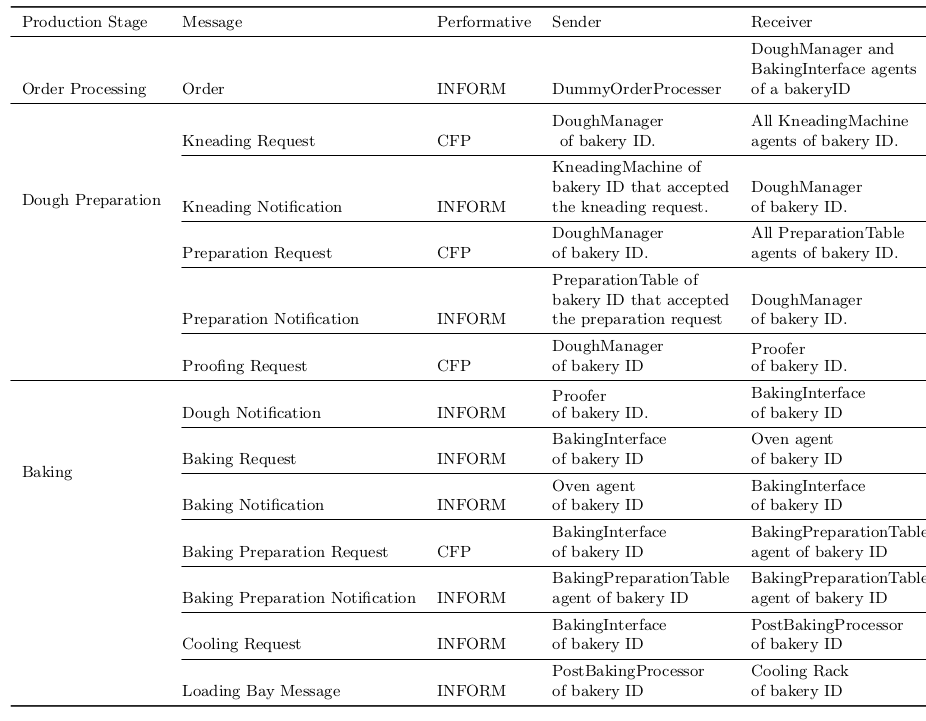
\includegraphics[scale=0.29]{images/messages.png}
			\end{figure}
		\end{frame}
		
		\begin{frame}
			\frametitle{Visualization}
			
			\begin{figure}\vspace{-1cm}
				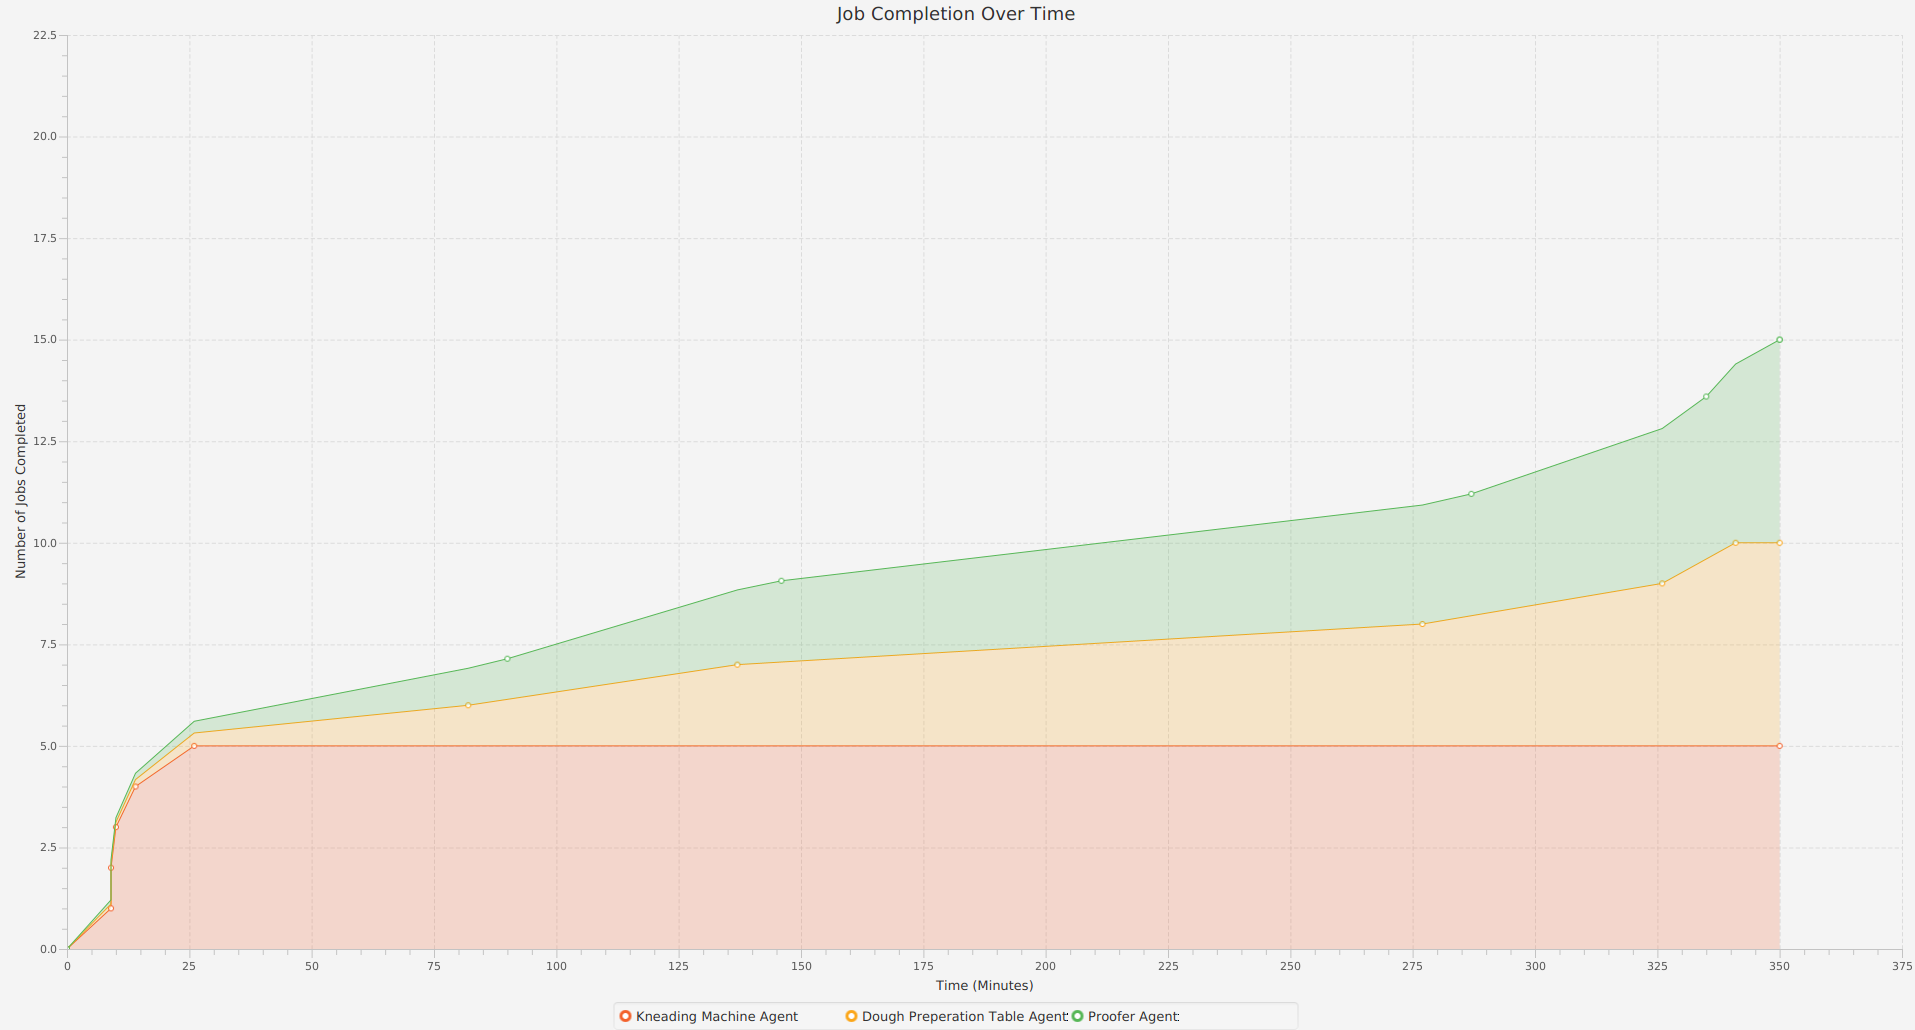
\includegraphics[scale=0.17`]{images/visualization.png}
			\end{figure}
		\end{frame}
		
		
\end{document}
